\documentclass[11pt]{article}

% Self-contained style matching the RadiationEffects_proj2 physics notes.
\usepackage[margin=1in]{geometry}
\usepackage[T1]{fontenc}
\usepackage[utf8]{inputenc}
\usepackage{lmodern}
\usepackage{microtype}
\usepackage[table]{xcolor}
\usepackage{amsmath,amssymb,amsfonts,mathtools,bm}
\usepackage{physics}
\usepackage{booktabs,array,longtable,tabularx}
\usepackage{hyperref}
\usepackage{enumitem}
\usepackage{fancyhdr}
\usepackage{titlesec}
\usepackage{tcolorbox}
\usepackage{ragged2e}
\usepackage{setspace}
\usepackage{siunitx}
\usepackage{tikz}
\usepackage{pgfplots}
\usepackage{float}
\usetikzlibrary{arrows.meta,positioning,shapes.geometric,calc,decorations.pathmorphing,patterns}
\pgfplotsset{compat=1.18}

\hypersetup{colorlinks=true, linkcolor=blue!50!black, urlcolor=blue!50!black, citecolor=blue!50!black}
\definecolor{TitleBlue}{HTML}{163A5F}
\definecolor{AccentTeal}{HTML}{2D6F73}
\definecolor{SoftBlue}{HTML}{EAF3F8}
\definecolor{SoftTeal}{HTML}{EDF8F6}
\definecolor{SoftGray}{HTML}{F5F7FA}
\definecolor{RuleGray}{HTML}{D7DEE8}
\pagestyle{fancy}
\fancyhf{}
\lhead{RadiationEffects\_proj2}
\rhead{BCS, GL, and TDGL Theory}
\cfoot{\thepage}
\setlength{\headheight}{14pt}
\setlength{\parskip}{0.5em}
\setlength{\parindent}{0pt}
\onehalfspacing
\numberwithin{equation}{section}
\titleformat{\section}{\Large\bfseries\color{TitleBlue}}{\thesection}{0.6em}{}
\titleformat{\subsection}{\large\bfseries\color{AccentTeal}}{\thesubsection}{0.6em}{}
\titleformat{\subsubsection}{\normalsize\bfseries\color{TitleBlue}}{\thesubsubsection}{0.6em}{}
\newtcolorbox{overviewbox}{colback=SoftBlue,colframe=TitleBlue,boxrule=0.8pt,arc=2mm,left=3mm,right=3mm,top=2mm,bottom=2mm}
\newtcolorbox{physicsbox}{colback=SoftTeal,colframe=AccentTeal,boxrule=0.8pt,arc=2mm,left=3mm,right=3mm,top=2mm,bottom=2mm}
\newtcolorbox{notebox}{colback=SoftGray,colframe=AccentTeal,boxrule=0.6pt,arc=2mm,left=3mm,right=3mm,top=2mm,bottom=2mm}
\newcommand{\DocTitle}[3]{%
\begin{center}
{\LARGE \bfseries \color{TitleBlue} #1}\\[0.5em]
{\large \color{AccentTeal} #2}\\[0.8em]
{\normalsize #3}
\end{center}
\vspace{0.5em}}
\newenvironment{symtable}{\rowcolors{2}{SoftGray}{white}\begin{longtable}{>{\RaggedRight\arraybackslash}p{0.18\textwidth} >{\RaggedRight\arraybackslash}p{0.25\textwidth} >{\RaggedRight\arraybackslash}p{0.47\textwidth}}\toprule \textbf{Symbol / acronym} & \textbf{Name} & \textbf{Meaning in this document} \\ \midrule\endfirsthead\toprule \textbf{Symbol / acronym} & \textbf{Name} & \textbf{Meaning in this document} \\ \midrule\endhead}{\bottomrule\end{longtable}}
\newcommand{\ProjectTOC}{\vspace{0.6em} {\hypersetup{linkcolor=TitleBlue,urlcolor=TitleBlue,citecolor=TitleBlue}\tableofcontents} \vspace{1.0em}}
\newcommand{\SymbolsAcronymsSection}{\section*{Symbols and acronyms used in this document}\addcontentsline{toc}{section}{Symbols and acronyms used in this document}}
\newcommand{\kB}{k_{\mathrm{B}}}
\newcommand{\rvec}{\bm{r}}
\newcommand{\qvec}{\bm{q}}
\newcommand{\kvec}{\bm{k}}
\newcommand{\kvecp}{\bm{k}^{\prime}}
\newcommand{\pvec}{\bm{p}}
\newcommand{\Avec}{\bm{A}}
\newcommand{\Evec}{\bm{E}}
\newcommand{\Bvec}{\bm{B}}
\newcommand{\Jvec}{\bm{J}}
\newcommand{\nvec}{\bm{n}}
\newcommand{\vvec}{\bm{v}}
\renewcommand{\grad}{\bm{\nabla}}
\newcommand{\lap}{\nabla^2}
\providecommand{\ii}{\mathrm{i}}
\providecommand{\ee}{\mathrm{e}}
\renewcommand{\dd}{\mathrm{d}}
\newcommand{\Tc}{T_{\mathrm{c}}}
\newcommand{\Tf}{T_{\mathrm{F}}}
\newcommand{\EF}{E_{\mathrm{F}}}
\newcommand{\xiGL}{\xi_{\mathrm{GL}}}
\newcommand{\lambdaL}{\lambda_{\mathrm{L}}}
\newcommand{\Phizero}{\Phi_0}
\newcommand{\Deltaz}{\Delta_0}
\newcommand{\Nzero}{N(0)}
\newcommand{\DOS}{\mathcal{N}}
\newcommand{\Ord}{\Psi}
\newcommand{\Op}{\hat{\Delta}}
\newcommand{\FGL}{\mathcal{F}}
\newcommand{\fGL}{f}
\newcommand{\jpair}{\bm{j}_{\mathrm{s}}}
\newcommand{\GammaTD}{\Gamma}
\allowdisplaybreaks

\begin{document}

\DocTitle{BCS Theory, Ginzburg-Landau Theory, and Time-Dependent Ginzburg-Landau Theory}{Derivation-Focused Physics Note for \texttt{RadiationEffects\_proj2}}{Microscopic pairing, macroscopic order-parameter theory, and dynamical superconducting response for radiation-effects modeling}

\begin{overviewbox}
\textbf{Purpose of this note.} This note gives a textbook-style derivation of three levels of superconductivity theory used in superconducting-device radiation modeling: BCS theory, Ginzburg-Landau theory, and time-dependent Ginzburg-Landau theory. The goal is not merely to list equations. The goal is to show how the equations arise, what each approximation means physically, and how the theories connect to quantities that matter for superconducting qubits and radiation-effects simulations: the energy gap, quasiparticle density, condensate phase, coherence length, penetration depth, vortex physics, pair breaking, relaxation of the order parameter, and electromagnetic coupling.
\end{overviewbox}

\ProjectTOC

\SymbolsAcronymsSection
\begin{symtable}
BCS & Bardeen-Cooper-Schrieffer theory & Microscopic theory in which an effective attractive interaction near the Fermi surface produces Cooper pairs and a gapped quasiparticle spectrum. \\
GL & Ginzburg-Landau theory & Phenomenological order-parameter theory obtained by expanding the free energy near the superconducting transition temperature. \\
TDGL & Time-dependent Ginzburg-Landau theory & Dynamical extension of GL theory that evolves the order parameter toward local free-energy extrema while preserving gauge covariance. \\
SC & Superconducting & Condensed state with macroscopic phase coherence, an excitation gap, flux quantization, and nondissipative supercurrent in ideal equilibrium. \\
QP & Quasiparticle & Excited state above the superconducting condensate; in BCS theory it is a coherent electron-hole mixture. \\
CP & Cooper pair & Bound, correlated pair of electrons with opposite momenta and opposite spins in the simplest spin-singlet BCS state. \\
$\rvec$ & Position & Real-space coordinate. \\
$\kvec$ & Crystal momentum & Wave vector labeling single-particle states in the normal metal or quasiparticle states in the superconductor. \\
$\sigma$ & Spin index & Spin projection, usually $\uparrow$ or $\downarrow$. \\
$\epsilon_{\kvec}$ & Single-particle energy & Band energy measured from a chosen zero. \\
$\xi_{\kvec}$ & Energy from Fermi level & $\xi_{\kvec}=\epsilon_{\kvec}-\mu$, with chemical potential $\mu$. \\
$\EF$ & Fermi energy & Characteristic electronic energy scale of the normal metal. \\
$\omega_D$ & Debye frequency & Phonon cutoff frequency in the simple BCS model. \\
$V$ & Pairing strength & Magnitude of the effective attractive interaction in the reduced BCS Hamiltonian. \\
$\Nzero$ & Density of states at Fermi level & Single-particle density of states per spin or total density of states depending on convention; the convention is stated when used. \\
$\Delta$ & Superconducting gap & BCS pair potential and minimum quasiparticle excitation energy in the isotropic $s$-wave case. \\
$\Deltaz$ & Zero-temperature gap & Energy gap at $T=0$. \\
$u_{\kvec},v_{\kvec}$ & Coherence factors & BCS amplitudes describing empty and pair-occupied components of state $(\kvec,-\kvec)$. \\
$E_{\kvec}$ & Quasiparticle energy & $E_{\kvec}=\sqrt{\xi_{\kvec}^2+|\Delta|^2}$. \\
$\Tc$ & Critical temperature & Temperature below which the superconducting state becomes stable. \\
$\Ord$ & GL order parameter & Complex macroscopic order parameter whose magnitude measures condensate amplitude and whose phase carries supercurrent. \\
$\alpha,\beta$ & GL coefficients & Phenomenological expansion coefficients in $f=\alpha |\Ord|^2+\beta |\Ord|^4/2+\cdots$. \\
$\alpha_0$ & GL temperature slope & Coefficient in $\alpha(T)=\alpha_0(T-\Tc)$ near $\Tc$. \\
$m^*$ & Pair effective mass & Effective mass associated with the GL order parameter; often $m^*\approx 2m_e$ in simple continuum notation. \\
$q^*$ & Pair charge & Charge of the GL condensate; for electron Cooper pairs $q^*=-2e$, while many formulae use the magnitude $2e$. \\
$\Avec$ & Vector potential & Magnetic vector potential with $\Bvec=\grad\times\Avec$. \\
$\phi$ & Scalar potential & Electric scalar potential. \\
$\Phizero$ & Flux quantum & $\Phizero=h/(2e)$ for Cooper pairs. \\
$\xiGL$ & GL coherence length & Length scale over which the order-parameter amplitude heals. \\
$\lambdaL$ & London penetration depth & Magnetic-field screening length. \\
$\kappa$ & GL parameter & $\kappa=\lambdaL/\xiGL$, controlling type-I versus type-II behavior. \\
$H_c$ & Thermodynamic critical field & Field scale at which uniform normal and superconducting phases have equal free energy in type-I theory. \\
$H_{c1},H_{c2}$ & Lower and upper critical fields & Field scales for vortex entry and destruction of superconductivity in a type-II superconductor. \\
$\GammaTD$ & TDGL relaxation coefficient & Coefficient controlling order-parameter relaxation dynamics. \\
$\tau_{\mathrm{GL}}$ & GL relaxation time & Characteristic time scale for small-amplitude order-parameter relaxation near $\Tc$. \\
$\mu$ & Chemical potential & Thermodynamic energy cost to add particles. \\
$\mu^*$ & Charge-imbalance potential & Nonequilibrium quasiparticle chemical-potential-like variable in reduced nonequilibrium superconductivity models. \\
\end{symtable}

\section{Why these three theories are all needed}

Superconductivity has several correct descriptions, but they answer different questions. BCS theory is microscopic. It explains how an attractive interaction between electrons near the Fermi surface destabilizes the normal Fermi sea, produces Cooper pairs, opens a gap, and creates quasiparticles. GL theory is macroscopic. It does not begin with the electron Hamiltonian. It begins with a complex order parameter and writes the most general local free energy allowed by symmetry near the transition temperature. TDGL adds dynamics to the GL order parameter. It describes relaxation of the condensate amplitude and phase after a perturbation, especially near $\Tc$ and in dirty gapless limits where a local relaxation equation is meaningful.

For radiation-effects modeling in superconducting devices, one should not treat these theories as interchangeable. They form a hierarchy:
\begin{equation}
\boxed{\text{microscopic pairing and QPs} \longrightarrow \text{order-parameter free energy} \longrightarrow \text{order-parameter dynamics}.}
\end{equation}

\begin{center}
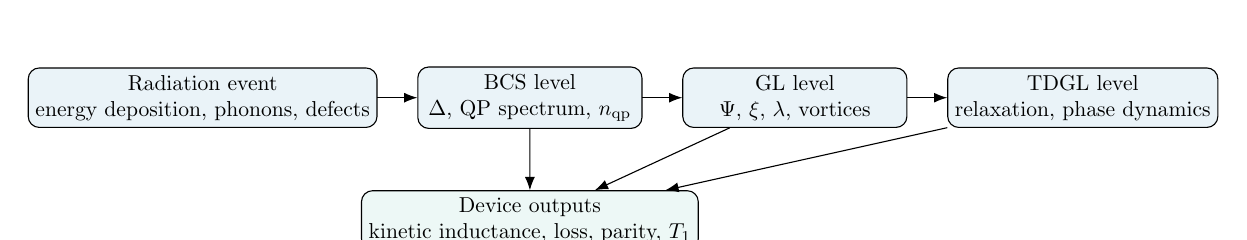
\begin{tikzpicture}[node distance=0.55cm,>=Latex,scale=0.78,transform shape]
\tikzstyle{blk}=[draw,rounded corners,align=center,minimum width=3.65cm,minimum height=0.95cm,fill=SoftBlue]
\tikzstyle{smallblk}=[draw,rounded corners,align=center,minimum width=3.5cm,minimum height=0.9cm,fill=SoftTeal]
\node[blk] (rad) {Radiation event\\energy deposition, phonons, defects};
\node[blk,right=0.65cm of rad] (bcs) {BCS level\\$\Delta$, QP spectrum, $n_{\mathrm{qp}}$};
\node[blk,right=0.65cm of bcs] (gl) {GL level\\$\Psi$, $\xi$, $\lambda$, vortices};
\node[blk,right=0.65cm of gl] (tdgl) {TDGL level\\relaxation, phase dynamics};
\node[smallblk,below=1.0cm of bcs] (device) {Device outputs\\kinetic inductance, loss, parity, $T_1$};
\draw[->] (rad)--(bcs);
\draw[->] (bcs)--(gl);
\draw[->] (gl)--(tdgl);
\draw[->] (bcs)--(device);
\draw[->] (gl)--(device);
\draw[->] (tdgl)--(device);
\end{tikzpicture}
\end{center}

\begin{physicsbox}
\textbf{Interpretation for this project.} BCS theory tells us what the superconducting gap is and how many quasiparticles are produced. GL theory tells us how the condensate amplitude and phase respond spatially to fields, boundaries, defects, and geometry. TDGL tells us how the order parameter can recover or be suppressed after a transient perturbation. A radiation event can therefore enter at all three levels: by breaking pairs, by changing material coefficients, and by driving nonequilibrium dynamics.
\end{physicsbox}

\section{Normal electrons, the Fermi surface, and why pairing is surprising}

\subsection{The normal Fermi gas}

Begin with noninteracting electrons in a volume $\mathcal{V}$, represented by creation and annihilation operators $c_{\kvec\sigma}^{\dagger}$ and $c_{\kvec\sigma}$. The normal-state Hamiltonian is
\begin{equation}
H_0=\sum_{\kvec,\sigma}\epsilon_{\kvec} c_{\kvec\sigma}^{\dagger}c_{\kvec\sigma}.
\end{equation}
In the grand-canonical ensemble it is more convenient to subtract the chemical potential term $\mu N$:
\begin{equation}
K_0=H_0-\mu N=\sum_{\kvec,\sigma}\xi_{\kvec} c_{\kvec\sigma}^{\dagger}c_{\kvec\sigma},
\qquad
\xi_{\kvec}=\epsilon_{\kvec}-\mu.
\end{equation}
At $T=0$ the normal ground state is the filled Fermi sea:
\begin{equation}
\ket{\mathrm{FS}}=\prod_{|\kvec|<k_F} c_{\kvec\uparrow}^{\dagger}c_{\kvec\downarrow}^{\dagger}\ket{0}.
\end{equation}
All states below the Fermi surface are occupied and all states above it are empty. Ordinary low-energy excitations are particle-hole excitations near the Fermi surface.

The naive expectation is that weak interactions only slightly perturb this Fermi liquid. Superconductivity is surprising because an arbitrarily weak attractive interaction in the Cooper channel destabilizes the Fermi surface. The instability is not a small correction. It reorganizes the many-body ground state and opens an energy gap.

\subsection{Effective attraction from phonons: what is kept in reduced BCS theory}

The microscopic source of attraction in conventional superconductors is electron-phonon coupling. A schematic electron-phonon Hamiltonian is
\begin{equation}
H=\sum_{\kvec\sigma}\epsilon_{\kvec} c_{\kvec\sigma}^{\dagger}c_{\kvec\sigma}
+\sum_{\qvec}\hbar\omega_{\qvec} b_{\qvec}^{\dagger}b_{\qvec}
+\sum_{\kvec\qvec\sigma}g_{\qvec} c_{\kvec+\qvec,\sigma}^{\dagger}c_{\kvec\sigma}(b_{\qvec}+b_{-\qvec}^{\dagger}).
\end{equation}
Here $b_{\qvec}^{\dagger}$ creates a phonon. If phonons are integrated out at second order, one obtains an effective electron-electron interaction. The rough structure is
\begin{equation}
V_{\mathrm{eff}}(\qvec,\omega)\sim |g_{\qvec}|^2\frac{2\hbar\omega_{\qvec}}{(\hbar\omega)^2-(\hbar\omega_{\qvec})^2}.
\end{equation}
At small exchanged frequency compared with the phonon frequency, the denominator is negative, so the phonon-mediated part is attractive:
\begin{equation}
V_{\mathrm{eff}}\sim -\frac{2|g_{\qvec}|^2}{\hbar\omega_{\qvec}}.
\end{equation}
This does not mean all Coulomb repulsion vanishes. Rather, the retarded phonon attraction can overcome the screened Coulomb repulsion in a narrow shell around the Fermi surface.

Reduced BCS theory keeps only the pairing part of this interaction:
\begin{equation}
K_{\mathrm{BCS}}=\sum_{\kvec\sigma}\xi_{\kvec} c_{\kvec\sigma}^{\dagger}c_{\kvec\sigma}
-\sum_{\kvec\kvecp}V_{\kvec\kvecp}
 c_{\kvec\uparrow}^{\dagger}c_{-\kvec\downarrow}^{\dagger}c_{-\kvecp\downarrow}c_{\kvecp\uparrow}.
\label{eq:reduced_bcs}
\end{equation}
In the simplest $s$-wave model,
\begin{equation}
V_{\kvec\kvecp}=
\begin{cases}
V>0, & |\xi_{\kvec}|<\hbar\omega_D,\quad |\xi_{\kvecp}|<\hbar\omega_D,\\
0, & \text{otherwise},
\end{cases}
\end{equation}
and the minus sign in Eq.~\eqref{eq:reduced_bcs} makes the interaction attractive.

\begin{notebox}
\textbf{Important approximation.} The reduced BCS Hamiltonian is not the full electron-electron Hamiltonian. It selects scattering processes in which a pair $(\kvec\uparrow,-\kvec\downarrow)$ scatters into another pair $(\kvecp\uparrow,-\kvecp\downarrow)$. This selection is justified because the superconducting instability occurs in this time-reversed-pair channel.
\end{notebox}

\section{The Cooper problem: one pair above a filled Fermi sea}

\subsection{Two-particle ansatz}

Before the full many-body BCS state, consider the Cooper problem: two electrons are added above an inert filled Fermi sea and interact attractively. Use the spin-singlet, zero-center-of-mass ansatz
\begin{equation}
\ket{\psi}=\sum_{\kvec>k_F} a_{\kvec} c_{\kvec\uparrow}^{\dagger}c_{-\kvec\downarrow}^{\dagger}\ket{\mathrm{FS}}.
\end{equation}
The condition $\kvec>k_F$ means the pair occupies states above the filled sea, because lower states are Pauli blocked. Let the pair energy relative to the filled Fermi sea be $E$. Acting with the Hamiltonian gives
\begin{equation}
(2\xi_{\kvec}-E)a_{\kvec}=\sum_{\kvecp}V_{\kvec\kvecp}a_{\kvecp}.
\end{equation}
For a constant attractive interaction $V_{\kvec\kvecp}=V$ inside the phonon shell and zero otherwise, the right side is independent of $\kvec$:
\begin{equation}
C\equiv V\sum_{\kvecp}a_{\kvecp}.
\end{equation}
Thus
\begin{equation}
a_{\kvec}=\frac{C}{2\xi_{\kvec}-E}.
\end{equation}
Summing over $\kvec$ and using the definition of $C$ gives
\begin{equation}
C=V\sum_{\kvec} \frac{C}{2\xi_{\kvec}-E}.
\end{equation}
For a nonzero solution, $C\ne 0$, so
\begin{equation}
1=V\sum_{0<\xi_{\kvec}<\hbar\omega_D}\frac{1}{2\xi_{\kvec}-E}.
\end{equation}

\subsection{Binding energy}

Replace the sum by a density-of-states integral. If $\Nzero$ is the single-spin density of states at the Fermi level and is approximately constant in the shell,
\begin{equation}
1=V\Nzero\int_0^{\hbar\omega_D}\frac{d\xi}{2\xi-E}.
\end{equation}
A bound state has $E<0$. Write $E=-\epsilon_b$, with $\epsilon_b>0$:
\begin{equation}
1=V\Nzero\int_0^{\hbar\omega_D}\frac{d\xi}{2\xi+\epsilon_b}.
\end{equation}
The integral is elementary:
\begin{align}
\int_0^{\hbar\omega_D}\frac{d\xi}{2\xi+\epsilon_b}
&=\frac{1}{2}\ln(2\xi+\epsilon_b)\bigg|_0^{\hbar\omega_D}\\
&=\frac{1}{2}\ln\left(\frac{2\hbar\omega_D+\epsilon_b}{\epsilon_b}\right).
\end{align}
Therefore
\begin{equation}
1=\frac{V\Nzero}{2}\ln\left(\frac{2\hbar\omega_D+\epsilon_b}{\epsilon_b}\right).
\end{equation}
In weak coupling, $\epsilon_b\ll 2\hbar\omega_D$, so
\begin{equation}
1\approx \frac{V\Nzero}{2}\ln\left(\frac{2\hbar\omega_D}{\epsilon_b}\right).
\end{equation}
Solving,
\begin{equation}
\epsilon_b\approx 2\hbar\omega_D\exp\left[-\frac{2}{V\Nzero}\right].
\label{eq:cooper_binding}
\end{equation}

\begin{physicsbox}
\textbf{Physical lesson of the Cooper problem.} The binding energy is nonzero for any attractive $V>0$, even if $V$ is arbitrarily weak. The exponential dependence means the energy scale is tiny compared with electronic scales, but the Fermi surface is unstable. This is the seed of superconductivity.
\end{physicsbox}

\section{The BCS variational state}

\subsection{Pair occupation as a two-level problem}

For each pair of time-reversed states $(\kvec\uparrow,-\kvec\downarrow)$, the BCS ground state mixes two possibilities:
\begin{itemize}[leftmargin=2em]
\item the pair state is empty,
\item the pair state is occupied by two electrons.
\end{itemize}
The variational state is
\begin{equation}
\ket{\mathrm{BCS}}=\prod_{\kvec} \left(u_{\kvec}+v_{\kvec} c_{\kvec\uparrow}^{\dagger}c_{-\kvec\downarrow}^{\dagger}\right)\ket{0},
\label{eq:bcs_state}
\end{equation}
with
\begin{equation}
|u_{\kvec}|^2+|v_{\kvec}|^2=1.
\end{equation}
The product form works because pair operators for different $\kvec$ act on different single-particle states. The probability that pair state $\kvec$ is occupied is $|v_{\kvec}|^2$; the probability it is empty is $|u_{\kvec}|^2$.

A normal Fermi sea would have a sharp occupation:
\begin{equation}
|v_{\kvec}|^2=\begin{cases}1,& \xi_{\kvec}<0,\\0,&\xi_{\kvec}>0.\end{cases}
\end{equation}
The superconducting state smooths this occupation near the Fermi surface over an energy scale set by $\Delta$.

\subsection{Expectation value of the reduced Hamiltonian}

Assume $u_{\kvec}$ and $v_{\kvec}$ are real for now. The number expectation for a spin state is
\begin{equation}
\langle c_{\kvec\uparrow}^{\dagger}c_{\kvec\uparrow}\rangle=v_{\kvec}^2,
\qquad
\langle c_{-\kvec\downarrow}^{\dagger}c_{-\kvec\downarrow}\rangle=v_{\kvec}^2.
\end{equation}
Therefore the kinetic contribution in the grand-canonical Hamiltonian is
\begin{equation}
\langle K_0\rangle=2\sum_{\kvec} \xi_{\kvec} v_{\kvec}^2.
\end{equation}
The anomalous pair expectation value is
\begin{equation}
\langle c_{-\kvec\downarrow}c_{\kvec\uparrow}\rangle=u_{\kvec} v_{\kvec}.
\end{equation}
To see this explicitly, focus on a single pair state:
\begin{equation}
\ket{\psi_{\kvec}}=u_{\kvec}\ket{0}+v_{\kvec}\ket{\uparrow\downarrow}.
\end{equation}
Then
\begin{equation}
c_{-\kvec\downarrow}c_{\kvec\uparrow}\ket{\uparrow\downarrow}=\ket{0},
\qquad
c_{-\kvec\downarrow}c_{\kvec\uparrow}\ket{0}=0,
\end{equation}
so
\begin{equation}
\bra{\psi_{\kvec}}c_{-\kvec\downarrow}c_{\kvec\uparrow}\ket{\psi_{\kvec}}=u_{\kvec} v_{\kvec}.
\end{equation}
Using mean-field factorization for distinct pair states, the interaction energy is
\begin{equation}
\langle K_{\mathrm{int}}\rangle=-\sum_{\kvec\kvecp}V_{\kvec\kvecp}u_{\kvec} v_{\kvec} u_{\kvecp}v_{\kvecp}.
\end{equation}
Thus the variational energy is
\begin{equation}
E_{\mathrm{var}}=2\sum_{\kvec}\xi_{\kvec} v_{\kvec}^2-\sum_{\kvec\kvecp}V_{\kvec\kvecp}u_{\kvec} v_{\kvec} u_{\kvecp}v_{\kvecp}.
\label{eq:var_energy}
\end{equation}

\subsection{Definition of the gap}

Define the gap parameter
\begin{equation}
\Delta_{\kvec}=\sum_{\kvecp}V_{\kvec\kvecp}u_{\kvecp}v_{\kvecp}.
\label{eq:gap_definition}
\end{equation}
For an isotropic $s$-wave interaction, $\Delta_{\kvec}=\Delta$ inside the pairing shell.

Substituting this definition into the variation is useful because the interaction term is controlled by $u_{\kvec} v_{\kvec}$, the anomalous pair amplitude. The superconducting gap is therefore not just an excitation energy. It is also the self-consistent field generated by coherent pair correlations.

\subsection{Minimization with respect to pair amplitudes}

Enforce $u_{\kvec}^2+v_{\kvec}^2=1$ by parameterizing
\begin{equation}
u_{\kvec}=\cos\theta_{\kvec},
\qquad
v_{\kvec}=\sin\theta_{\kvec}.
\end{equation}
Then
\begin{equation}
v_{\kvec}^2=\frac{1-\cos 2\theta_{\kvec}}{2},
\qquad
u_{\kvec} v_{\kvec}=\frac{1}{2}\sin 2\theta_{\kvec}.
\end{equation}
Using Eq.~\eqref{eq:var_energy}, vary with respect to $\theta_{\kvec}$. The derivative of the kinetic term is
\begin{equation}
\frac{\partial}{\partial\theta_{\kvec}}\left(2\xi_{\kvec} v_{\kvec}^2\right)=4\xi_{\kvec} u_{\kvec} v_{\kvec}.
\end{equation}
The interaction term derivative gives
\begin{equation}
-2\Delta_{\kvec}\frac{\partial}{\partial\theta_{\kvec}}(u_{\kvec} v_{\kvec})
=-2\Delta_{\kvec}(u_{\kvec}^2-v_{\kvec}^2).
\end{equation}
Setting the variation to zero gives
\begin{equation}
4\xi_{\kvec} u_{\kvec} v_{\kvec}-2\Delta_{\kvec}(u_{\kvec}^2-v_{\kvec}^2)=0.
\end{equation}
Divide by 2:
\begin{equation}
2\xi_{\kvec} u_{\kvec} v_{\kvec}=\Delta_{\kvec}(u_{\kvec}^2-v_{\kvec}^2).
\label{eq:min_condition}
\end{equation}
The solution is expressed through the quasiparticle energy
\begin{equation}
E_{\kvec}=\sqrt{\xi_{\kvec}^2+|\Delta_{\kvec}|^2}.
\end{equation}
The coherence factors are
\begin{align}
u_{\kvec}^2&=\frac{1}{2}\left(1+\frac{\xi_{\kvec}}{E_{\kvec}}\right),\\
v_{\kvec}^2&=\frac{1}{2}\left(1-\frac{\xi_{\kvec}}{E_{\kvec}}\right),\\
u_{\kvec} v_{\kvec}&=\frac{\Delta_{\kvec}}{2E_{\kvec}}.
\end{align}
Check that these solve Eq.~\eqref{eq:min_condition}:
\begin{equation}
2\xi_{\kvec} u_{\kvec} v_{\kvec}=2\xi_{\kvec}\frac{\Delta_{\kvec}}{2E_{\kvec}}=\frac{\xi_{\kvec}\Delta_{\kvec}}{E_{\kvec}},
\end{equation}
and
\begin{equation}
\Delta_{\kvec}(u_{\kvec}^2-v_{\kvec}^2)=\Delta_{\kvec}\frac{\xi_{\kvec}}{E_{\kvec}}=\frac{\xi_{\kvec}\Delta_{\kvec}}{E_{\kvec}}.
\end{equation}

\subsection{The zero-temperature gap equation}

Insert $u_{\kvec} v_{\kvec}=\Delta_{\kvec}/(2E_{\kvec})$ into Eq.~\eqref{eq:gap_definition}. For a constant $s$-wave gap,
\begin{equation}
\Delta=V\sum_{|\xi_{\kvec}|<\hbar\omega_D}\frac{\Delta}{2\sqrt{\xi_{\kvec}^2+\Delta^2}}.
\end{equation}
For $\Delta\ne 0$,
\begin{equation}
1=V\sum_{|\xi_{\kvec}|<\hbar\omega_D}\frac{1}{2\sqrt{\xi_{\kvec}^2+\Delta^2}}.
\end{equation}
Replace the sum by a density-of-states integral. With $\Nzero$ the single-spin density of states and with symmetric integration around the Fermi level,
\begin{align}
1&=V\Nzero\int_{-\hbar\omega_D}^{\hbar\omega_D}\frac{d\xi}{2\sqrt{\xi^2+\Delta^2}}\\
&=V\Nzero\int_0^{\hbar\omega_D}\frac{d\xi}{\sqrt{\xi^2+\Delta^2}}.
\end{align}
The integral is
\begin{equation}
\int_0^{\hbar\omega_D}\frac{d\xi}{\sqrt{\xi^2+\Delta^2}}
=\sinh^{-1}\left(\frac{\hbar\omega_D}{\Delta}\right).
\end{equation}
In weak coupling, $\Delta\ll\hbar\omega_D$, so
\begin{equation}
\sinh^{-1}(x)=\ln(x+\sqrt{x^2+1})\approx \ln(2x),
\end{equation}
and
\begin{equation}
1\approx V\Nzero\ln\left(\frac{2\hbar\omega_D}{\Delta}\right).
\end{equation}
Therefore
\begin{equation}
\boxed{\Deltaz=2\hbar\omega_D\exp\left[-\frac{1}{V\Nzero}\right].}
\label{eq:zero_temp_gap}
\end{equation}

Compare this with the Cooper problem. The many-body BCS gap has an exponential scale $\exp[-1/(V\Nzero)]$, whereas the simple two-body Cooper binding energy carried $\exp[-2/(V\Nzero)]$ in Eq.~\eqref{eq:cooper_binding}. The many-body instability is stronger than a single isolated pair.

\section{Bogoliubov quasiparticles and the excitation gap}

\subsection{Mean-field Hamiltonian}

The reduced Hamiltonian can be approximated by replacing pair operators with their mean values plus fluctuations. Define
\begin{equation}
\Delta=V\sum_{\kvec}\langle c_{-\kvec\downarrow}c_{\kvec\uparrow}\rangle.
\end{equation}
The interaction term becomes
\begin{equation}
-\sum_{\kvec\kvecp}V c_{\kvec\uparrow}^{\dagger}c_{-\kvec\downarrow}^{\dagger}c_{-\kvecp\downarrow}c_{\kvecp\uparrow}
\approx
-\sum_{\kvec}\left(\Delta c_{\kvec\uparrow}^{\dagger}c_{-\kvec\downarrow}^{\dagger}+\Delta^* c_{-\kvec\downarrow}c_{\kvec\uparrow}\right)+\frac{|\Delta|^2}{V}.
\end{equation}
Thus
\begin{equation}
K_{\mathrm{MF}}=\sum_{\kvec}\xi_{\kvec}\left(c_{\kvec\uparrow}^{\dagger}c_{\kvec\uparrow}+c_{-\kvec\downarrow}^{\dagger}c_{-\kvec\downarrow}\right)
-\sum_{\kvec}\left(\Delta c_{\kvec\uparrow}^{\dagger}c_{-\kvec\downarrow}^{\dagger}+\Delta^* c_{-\kvec\downarrow}c_{\kvec\uparrow}\right)+\frac{|\Delta|^2}{V}.
\end{equation}
In Nambu spinor notation,
\begin{equation}
\Phi_{\kvec}=\begin{pmatrix}c_{\kvec\uparrow}\\c_{-\kvec\downarrow}^{\dagger}\end{pmatrix},
\end{equation}
the quadratic part is, up to a constant,
\begin{equation}
K_{\mathrm{MF}}=\sum_{\kvec} \Phi_{\kvec}^{\dagger}
\begin{pmatrix}
\xi_{\kvec} & -\Delta\\
-\Delta^* & -\xi_{\kvec}
\end{pmatrix}
\Phi_{\kvec}+\frac{|\Delta|^2}{V}+\text{constant}.
\end{equation}
The eigenvalues of the $2\times 2$ matrix satisfy
\begin{equation}
\det\begin{pmatrix}
\xi_{\kvec}-E & -\Delta\\
-\Delta^* & -\xi_{\kvec}-E
\end{pmatrix}=0.
\end{equation}
Compute the determinant:
\begin{equation}
(\xi_{\kvec}-E)(-\xi_{\kvec}-E)-|\Delta|^2=E^2-\xi_{\kvec}^2-|\Delta|^2=0.
\end{equation}
Therefore
\begin{equation}
\boxed{E_{\kvec}=\sqrt{\xi_{\kvec}^2+|\Delta|^2}.}
\end{equation}

\subsection{Bogoliubov transformation}

Introduce quasiparticle operators
\begin{align}
\gamma_{\kvec\uparrow}&=u_{\kvec} c_{\kvec\uparrow}-v_{\kvec} c_{-\kvec\downarrow}^{\dagger},\\
\gamma_{-\kvec\downarrow}^{\dagger}&=v_{\kvec} c_{\kvec\uparrow}+u_{\kvec} c_{-\kvec\downarrow}^{\dagger}.
\end{align}
The inverse transformation is
\begin{align}
c_{\kvec\uparrow}&=u_{\kvec}\gamma_{\kvec\uparrow}+v_{\kvec}\gamma_{-\kvec\downarrow}^{\dagger},\\
c_{-\kvec\downarrow}^{\dagger}&=-v_{\kvec}\gamma_{\kvec\uparrow}+u_{\kvec}\gamma_{-\kvec\downarrow}^{\dagger}.
\end{align}
Choosing the same coherence factors as before diagonalizes the mean-field Hamiltonian:
\begin{equation}
K_{\mathrm{MF}}=E_{\mathrm{GS}}+\sum_{\kvec,\sigma}E_{\kvec}\gamma_{\kvec\sigma}^{\dagger}\gamma_{\kvec\sigma}.
\end{equation}
The energy cost to create one quasiparticle is at least $|\Delta|$, because $E_{\kvec}$ is minimum at $\xi_{\kvec}=0$:
\begin{equation}
E_{\min}=|\Delta|.
\end{equation}
Breaking a Cooper pair creates two quasiparticles, so the pair-breaking threshold is approximately
\begin{equation}
\boxed{E_{\mathrm{pair\;break}}\ge 2\Delta.}
\end{equation}

\begin{physicsbox}
\textbf{Radiation-effects meaning.} A phonon, photon, or deposited energy branch that can deliver energy $\ge 2\Delta$ to the superconducting electronic system can break Cooper pairs. This is why high-energy phonons created by radiation interactions are relevant to quasiparticle poisoning in superconducting devices.
\end{physicsbox}

\section{BCS density of states and quasiparticle density}

\subsection{Derivation of the superconducting density of states}

The normal density of states near the Fermi level is approximately constant, $\DOS_n(E)\approx \Nzero$. In the superconducting state, the quasiparticle energy is
\begin{equation}
E=\sqrt{\xi^2+\Delta^2}.
\end{equation}
Solving for $\xi$ gives
\begin{equation}
\xi=\pm\sqrt{E^2-\Delta^2}.
\end{equation}
The density of states transforms according to
\begin{equation}
\DOS_s(E)dE=\DOS_n(\xi)d\xi.
\end{equation}
For each branch,
\begin{equation}
\left|\frac{d\xi}{dE}\right|=\frac{E}{\sqrt{E^2-\Delta^2}}.
\end{equation}
Therefore the superconducting quasiparticle density of states is
\begin{equation}
\boxed{\DOS_s(E)=\DOS_n(0)\frac{|E|}{\sqrt{E^2-\Delta^2}}\,\Theta(|E|-\Delta).}
\label{eq:bcs_dos}
\end{equation}
The step function $\Theta$ enforces the gap: there are no quasiparticle states for $|E|<\Delta$ in ideal clean $s$-wave BCS theory.

\begin{figure}[H]
\centering
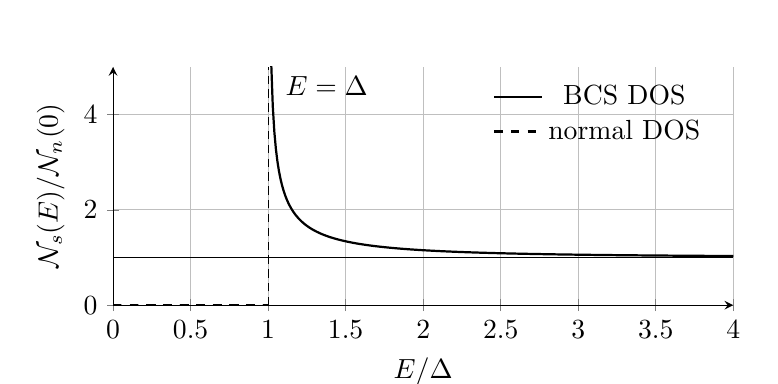
\begin{tikzpicture}
\begin{axis}[
width=0.78\textwidth,
height=0.38\textwidth,
xlabel={$E/\Delta$},
ylabel={$\DOS_s(E)/\DOS_n(0)$},
xmin=0,xmax=4,
ymin=0,ymax=5,
axis lines=left,
grid=both,
legend style={draw=none,fill=none,at={(0.97,0.97)},anchor=north east},
samples=300]
\addplot[domain=1.02:4,thick] {x/sqrt(x^2-1)};
\addplot[domain=0:1,thick,dashed] {0};
\addlegendentry{BCS DOS}
\addplot[domain=0:4,thin] {1};
\addlegendentry{normal DOS}
\draw[densely dashed] (axis cs:1,0) -- (axis cs:1,5);
\node[anchor=south west] at (axis cs:1.05,4.2) {$E=\Delta$};
\end{axis}
\end{tikzpicture}
\caption{Ideal normalized BCS quasiparticle density of states. The square-root singularity at the gap edge is a consequence of the energy transformation $E=\sqrt{\xi^2+\Delta^2}$. Real materials have broadening from disorder, lifetime effects, inhomogeneity, and nonequilibrium processes.}
\end{figure}

\subsection{Equilibrium quasiparticle density at low temperature}

The quasiparticle number density is obtained by integrating the superconducting density of states multiplied by the Fermi occupation factor:
\begin{equation}
n_{\mathrm{qp}}=2\int_{\Delta}^{\infty} dE\,\DOS_s(E)f(E),
\end{equation}
where the factor 2 accounts for spin if $\DOS_s$ is single-spin. At low temperature, $\kB T\ll \Delta$, the Fermi function is approximately
\begin{equation}
f(E)=\frac{1}{e^{E/(\kB T)}+1}\approx e^{-E/(\kB T)}.
\end{equation}
Near the gap edge, write
\begin{equation}
E=\Delta+\epsilon,
\qquad
\epsilon\ll\Delta.
\end{equation}
Then
\begin{equation}
E^2-\Delta^2=(\Delta+\epsilon)^2-\Delta^2\approx 2\Delta\epsilon,
\end{equation}
and
\begin{equation}
\DOS_s(E)\approx \Nzero\frac{\Delta}{\sqrt{2\Delta\epsilon}}=\Nzero\sqrt{\frac{\Delta}{2\epsilon}}.
\end{equation}
Therefore
\begin{align}
n_{\mathrm{qp}}&\approx 2\Nzero\int_0^{\infty}d\epsilon\sqrt{\frac{\Delta}{2\epsilon}}\exp\left[-\frac{\Delta+\epsilon}{\kB T}\right]\\
&=2\Nzero e^{-\Delta/(\kB T)}\sqrt{\frac{\Delta}{2}}
\int_0^{\infty}d\epsilon\,\epsilon^{-1/2}e^{-\epsilon/(\kB T)}.
\end{align}
Use
\begin{equation}
\int_0^{\infty}d\epsilon\,\epsilon^{-1/2}e^{-\epsilon/(\kB T)}=\sqrt{\pi\kB T}.
\end{equation}
Thus
\begin{equation}
\boxed{n_{\mathrm{qp}}(T)\approx 2\Nzero\sqrt{\frac{\pi\Delta\kB T}{2}}\,e^{-\Delta/(\kB T)}.}
\end{equation}
Depending on whether $\Nzero$ is defined per spin or including both spins, the prefactor is often written equivalently as
\begin{equation}
\boxed{n_{\mathrm{qp}}(T)\approx 2N_0\sqrt{2\pi \kB T\Delta}\,e^{-\Delta/(\kB T)},}
\end{equation}
where $N_0$ is a common single-spin convention used in superconducting-device literature. The exponential dependence is the essential point.

\section{Finite-temperature BCS gap equation and critical temperature}

\subsection{Thermal quasiparticles reduce the anomalous average}

At finite temperature, quasiparticle states are thermally occupied. The anomalous expectation value becomes
\begin{equation}
\langle c_{-\kvec\downarrow}c_{\kvec\uparrow}\rangle
=\frac{\Delta}{2E_{\kvec}}\tanh\left(\frac{E_{\kvec}}{2\kB T}\right).
\end{equation}
Therefore the finite-temperature gap equation is
\begin{equation}
\boxed{1=V\sum_{|\xi_{\kvec}|<\hbar\omega_D}\frac{1}{2E_{\kvec}}\tanh\left(\frac{E_{\kvec}}{2\kB T}\right).}
\label{eq:finite_T_gap}
\end{equation}
Near the critical temperature, $\Delta\to 0$, so $E_{\kvec}\to |\xi_{\kvec}|$. Then Eq.~\eqref{eq:finite_T_gap} becomes
\begin{equation}
1=V\Nzero\int_0^{\hbar\omega_D}\frac{d\xi}{\xi}\tanh\left(\frac{\xi}{2\kB \Tc}\right).
\end{equation}
The standard weak-coupling evaluation gives
\begin{equation}
\kB\Tc=1.14\,\hbar\omega_D\exp\left[-\frac{1}{V\Nzero}\right].
\end{equation}
Combining this with the zero-temperature gap from Eq.~\eqref{eq:zero_temp_gap},
\begin{equation}
\boxed{\frac{2\Deltaz}{\kB\Tc}\approx 3.53.}
\end{equation}
This number is a classic weak-coupling BCS result for an isotropic $s$-wave superconductor.

\subsection{Approximate gap temperature dependence}

A useful interpolation formula is
\begin{equation}
\Delta(T)\approx \Deltaz\tanh\left[1.74\sqrt{\frac{\Tc}{T}-1}\right].
\end{equation}
Near $\Tc$, the gap scales as
\begin{equation}
\Delta(T)\propto (1-T/\Tc)^{1/2}.
\end{equation}
This square-root behavior is the same critical exponent that appears in mean-field GL theory.

\begin{figure}[H]
\centering
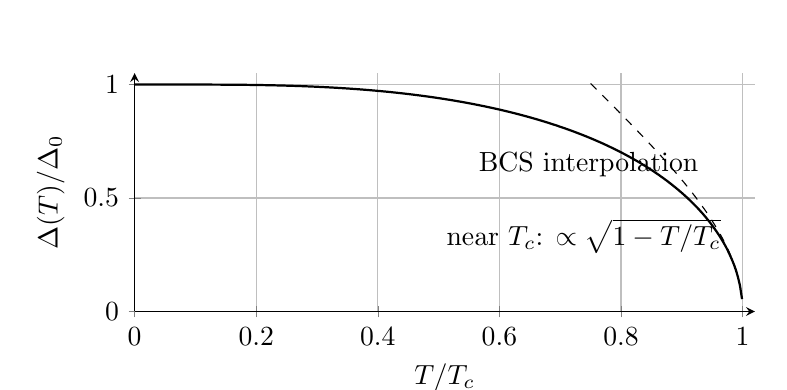
\begin{tikzpicture}
\begin{axis}[
width=0.78\textwidth,
height=0.38\textwidth,
xlabel={$T/T_c$},
ylabel={$\Delta(T)/\Delta_0$},
xmin=0,xmax=1.02,
ymin=0,ymax=1.05,
axis lines=left,
grid=both,
samples=300]
\addplot[domain=0.001:0.999,thick] {tanh(1.74*sqrt(1/x-1))};
\addplot[domain=0.75:0.999,dashed] {1.74*sqrt(1/x-1)};
\node[anchor=south west] at (axis cs:0.55,0.55) {BCS interpolation};
\node[anchor=north east] at (axis cs:0.98,0.45) {near $T_c$: $\propto\sqrt{1-T/T_c}$};
\end{axis}
\end{tikzpicture}
\caption{Approximate temperature dependence of the weak-coupling BCS gap. The gap closes continuously at $T_c$. Near $T_c$, the order parameter has mean-field square-root scaling.}
\end{figure}

\section{Condensation energy and why the superconducting state wins}

\subsection{Energy difference at zero temperature}

The superconducting state is stable because the reduction in interaction energy exceeds the kinetic-energy cost of smearing the Fermi surface. The zero-temperature condensation energy per volume in weak-coupling BCS theory is
\begin{equation}
\boxed{f_s-f_n=-\frac{1}{2}\Nzero\Delta^2,}
\label{eq:condensation_energy}
\end{equation}
up to convention-dependent spin factors. Let us sketch the derivation.

The BCS ground-state energy relative to the normal state can be written as
\begin{equation}
E_s-E_n=2\sum_{\kvec}\xi_{\kvec}\left(v_{\kvec}^2-\Theta(-\xi_{\kvec})\right)-\frac{\Delta^2}{V}.
\end{equation}
The first term is the kinetic-energy cost relative to the sharp Fermi sea; the second term is the pairing-energy gain. Use the gap equation to eliminate $1/V$:
\begin{equation}
\frac{1}{V}=\Nzero\int_0^{\hbar\omega_D}\frac{d\xi}{\sqrt{\xi^2+\Delta^2}}.
\end{equation}
After performing the integrals and taking the weak-coupling limit, the leading result is Eq.~\eqref{eq:condensation_energy}. The negative sign means the superconducting state has lower free energy.

\subsection{Connection to thermodynamic critical field}

The magnetic energy density of a field $H$ in SI units is $\mu_0 H^2/2$. A thermodynamic critical field satisfies
\begin{equation}
\frac{\mu_0 H_c^2}{2}=f_n-f_s.
\end{equation}
Using Eq.~\eqref{eq:condensation_energy},
\begin{equation}
H_c^2\sim \frac{\Nzero\Delta^2}{\mu_0}.
\end{equation}
This relation shows that the critical field is tied to the condensation energy: magnetic field destroys superconductivity when the magnetic-energy cost of expelling the field exceeds the condensation-energy gain.

\section{From BCS to macroscopic phase stiffness}

\subsection{Order parameter and broken gauge symmetry}

The BCS state has a nonzero anomalous average
\begin{equation}
F_{\kvec}=\langle c_{-\kvec\downarrow}c_{\kvec\uparrow}\rangle.
\end{equation}
The gap is proportional to this anomalous average:
\begin{equation}
\Delta=V\sum_{\kvec} F_{\kvec}.
\end{equation}
A global superconducting phase can be assigned:
\begin{equation}
\Delta=|\Delta|e^{i\theta}.
\end{equation}
The phase is physically meaningful only through gauge-invariant combinations. Under an electromagnetic gauge transformation,
\begin{align}
\Avec &\to \Avec+\grad\chi,\\
\phi &\to \phi-\pdv{\chi}{t},\\
\theta &\to \theta+\frac{q^*}{\hbar}\chi,
\end{align}
where $q^*$ is the condensate charge. The gauge-invariant phase gradient is
\begin{equation}
\grad\theta-\frac{q^*}{\hbar}\Avec.
\end{equation}
For electron Cooper pairs, $q^*=-2e$; many engineering formulae use the magnitude $2e$ and absorb signs into current convention.

\subsection{Supercurrent from phase stiffness}

A slowly varying phase costs energy. The continuum phase-stiffness energy has the form
\begin{equation}
f_{\mathrm{phase}}=\frac{1}{2}\rho_s\left(\grad\theta-\frac{q^*}{\hbar}\Avec\right)^2,
\end{equation}
where $\rho_s$ is the superfluid stiffness. The supercurrent is obtained by varying the free energy with respect to $\Avec$:
\begin{equation}
\Jvec_s=-\frac{\delta F}{\delta \Avec}.
\end{equation}
This gives
\begin{equation}
\Jvec_s=\frac{q^*\rho_s}{\hbar}\left(\grad\theta-\frac{q^*}{\hbar}\Avec\right).
\end{equation}
Equivalently, with condensate density $n_s$ and pair mass $m^*$,
\begin{equation}
\Jvec_s=\frac{q^*\hbar}{m^*}|\Ord|^2\left(\grad\theta-\frac{q^*}{\hbar}\Avec\right).
\label{eq:phase_current}
\end{equation}
This is the bridge from microscopic BCS phase coherence to GL supercurrent.

\section{Ginzburg-Landau theory: constructing the free energy}

\subsection{Why a phenomenological expansion is possible}

Near $\Tc$, the superconducting order parameter is small. A continuous transition allows a power-series expansion of the free-energy density in the order parameter and its gradients. The order parameter is complex:
\begin{equation}
\Ord(\rvec)=|\Ord(\rvec)|e^{i\theta(\rvec)}.
\end{equation}
Gauge invariance forbids ordinary gradients $\grad\Ord$ from appearing alone in the electromagnetic problem. The gauge-covariant derivative is
\begin{equation}
\bm{D}=\grad-\frac{i q^*}{\hbar}\Avec.
\end{equation}
The GL free-energy functional is
\begin{equation}
\boxed{
F[\Ord,\Avec]=\int d^3r\left[\alpha|\Ord|^2+\frac{\beta}{2}|\Ord|^4+\frac{1}{2m^*}\left|\left(-i\hbar\grad-q^*\Avec\right)\Ord\right|^2+\frac{|\Bvec|^2}{2\mu_0}\right].}
\label{eq:gl_functional}
\end{equation}
The coefficient $\beta$ must be positive for stability. The coefficient $\alpha$ changes sign at $\Tc$:
\begin{equation}
\alpha(T)=\alpha_0(T-\Tc).
\end{equation}
For $T>\Tc$, $\alpha>0$ and the minimum is $\Ord=0$. For $T<\Tc$, $\alpha<0$ and the minimum is at nonzero $|\Ord|$.

\begin{figure}[H]
\centering
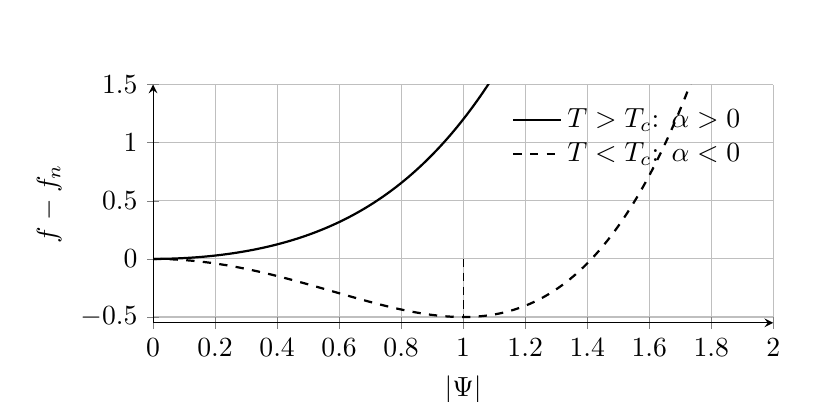
\begin{tikzpicture}
\begin{axis}[
width=0.78\textwidth,
height=0.38\textwidth,
xlabel={$|\Psi|$},
ylabel={$f-f_n$},
xmin=0,xmax=2.0,
ymin=-0.55,ymax=1.5,
axis lines=left,
grid=both,
legend style={draw=none,fill=none,at={(0.97,0.95)},anchor=north east},
samples=200]
\addplot[domain=0:2,thick] {0.7*x^2 + 0.5*x^4};
\addlegendentry{$T>T_c$: $\alpha>0$}
\addplot[domain=0:2,thick,dashed] {-1.0*x^2 + 0.5*x^4};
\addlegendentry{$T<T_c$: $\alpha<0$}
\draw[densely dashed] (axis cs:1,0) -- (axis cs:1,-0.5);
\node[anchor=north] at (axis cs:1,-0.5) {$|\Psi_0|$};
\end{axis}
\end{tikzpicture}
\caption{GL local free-energy density $f=\alpha|\Psi|^2+\beta |\Psi|^4/2$. Above $T_c$ the minimum is at $|\Psi|=0$. Below $T_c$ the minimum shifts to nonzero order-parameter amplitude.}
\end{figure}

\subsection{Uniform solution}

Ignore gradients and magnetic field. The local free-energy density relative to the normal state is
\begin{equation}
f_s-f_n=\alpha|\Ord|^2+\frac{\beta}{2}|\Ord|^4.
\end{equation}
Let $\rho=|\Ord|^2$. Then
\begin{equation}
f_s-f_n=\alpha\rho+\frac{\beta}{2}\rho^2.
\end{equation}
Minimize with respect to $\rho$:
\begin{equation}
\pdv{f}{\rho}=\alpha+\beta\rho=0.
\end{equation}
Thus
\begin{equation}
|\Ord_0|^2=\rho_0=-\frac{\alpha}{\beta},\qquad T<\Tc.
\label{eq:gl_uniform_order}
\end{equation}
The free-energy density at the minimum is
\begin{equation}
f_s-f_n=\alpha\left(-\frac{\alpha}{\beta}\right)+\frac{\beta}{2}\left(\frac{\alpha^2}{\beta^2}\right)
=-\frac{\alpha^2}{2\beta}.
\label{eq:gl_condensation}
\end{equation}
This is the GL condensation-energy density. Comparing to the magnetic energy density,
\begin{equation}
\frac{\mu_0H_c^2}{2}=\frac{\alpha^2}{2\beta},
\end{equation}
so
\begin{equation}
\boxed{H_c=\frac{|\alpha|}{\sqrt{\mu_0\beta}}.}
\end{equation}

\section{Deriving the GL equations}

\subsection{Variation with respect to $\Psi^*$}

The GL free energy contains
\begin{equation}
f=\alpha|\Ord|^2+\frac{\beta}{2}|\Ord|^4+\frac{1}{2m^*}|\hat{\Pi}\Ord|^2+\frac{|\Bvec|^2}{2\mu_0},
\end{equation}
where
\begin{equation}
\hat{\Pi}=-i\hbar\grad-q^*\Avec.
\end{equation}
Vary $F$ with respect to $\Ord^*$. The local terms vary as
\begin{equation}
\delta |\Ord|^2=\Ord\delta\Ord^*,
\qquad
\delta |\Ord|^4=2|\Ord|^2\Ord\delta\Ord^*.
\end{equation}
Therefore
\begin{equation}
\delta F_{\mathrm{local}}=\int d^3r\left(\alpha\Ord+\beta|\Ord|^2\Ord\right)\delta\Ord^*.
\end{equation}
The gradient term is
\begin{equation}
F_{\mathrm{grad}}=\int d^3r\frac{1}{2m^*}(\hat{\Pi}\Ord)^*(\hat{\Pi}\Ord).
\end{equation}
Varying with respect to $\Ord^*$ gives
\begin{equation}
\delta F_{\mathrm{grad}}=\int d^3r\frac{1}{2m^*}(\hat{\Pi}\delta\Ord)^*(\hat{\Pi}\Ord).
\end{equation}
After integration by parts, assuming boundary terms vanish or are handled by boundary conditions,
\begin{equation}
\delta F_{\mathrm{grad}}=\int d^3r\,\delta\Ord^*\frac{1}{2m^*}\hat{\Pi}^2\Ord.
\end{equation}
Setting $\delta F/\delta\Ord^*=0$ gives the first GL equation:
\begin{equation}
\boxed{\alpha\Ord+\beta|\Ord|^2\Ord+\frac{1}{2m^*}\left(-i\hbar\grad-q^*\Avec\right)^2\Ord=0.}
\label{eq:first_gl}
\end{equation}

\subsection{Boundary condition from the variation}

The integration by parts also produces a boundary term proportional to
\begin{equation}
\nvec\cdot\left(-i\hbar\grad-q^*\Avec\right)\Ord.
\end{equation}
For an insulating boundary with no supercurrent through the surface, the natural boundary condition is
\begin{equation}
\boxed{\nvec\cdot\left(-i\hbar\grad-q^*\Avec\right)\Ord=0.}
\label{eq:gl_neumann}
\end{equation}
This is the gauge-covariant version of a Neumann boundary condition.

\subsection{Variation with respect to the vector potential}

The supercurrent follows from the variation of the kinetic term with respect to $\Avec$. Write
\begin{equation}
\hat{\Pi}\Ord=(-i\hbar\grad-q^*\Avec)\Ord.
\end{equation}
A variation $\delta\Avec$ changes this by
\begin{equation}
\delta(\hat{\Pi}\Ord)=-q^*\delta\Avec\,\Ord.
\end{equation}
Then
\begin{align}
\delta F_{\mathrm{grad}}&=\int d^3r\frac{1}{2m^*}\left[(\delta\hat{\Pi}\Ord)^*(\hat{\Pi}\Ord)+(\hat{\Pi}\Ord)^*(\delta\hat{\Pi}\Ord)\right]\\
&=\int d^3r\frac{1}{2m^*}\left[-q^*\delta\Avec\,\Ord^*(\hat{\Pi}\Ord)-q^* (\hat{\Pi}\Ord)^*\delta\Avec\,\Ord\right]\\
&=-\int d^3r\,\delta\Avec\cdot\frac{q^*}{2m^*}\left[\Ord^*(\hat{\Pi}\Ord)+(\hat{\Pi}\Ord)^*\Ord\right].
\end{align}
Thus the supercurrent density is
\begin{equation}
\boxed{\Jvec_s=\frac{q^*}{2m^*}\left[\Ord^*(-i\hbar\grad-q^*\Avec)\Ord+\Ord(i\hbar\grad-q^*\Avec)\Ord^*\right].}
\label{eq:gl_current_general}
\end{equation}
This can be written as
\begin{equation}
\boxed{\Jvec_s=\frac{q^*\hbar}{2m^*i}\left(\Ord^*\grad\Ord-\Ord\grad\Ord^*\right)-\frac{(q^*)^2}{m^*}|\Ord|^2\Avec.}
\label{eq:gl_current}
\end{equation}
If $\Ord=|\Ord|e^{i\theta}$, then
\begin{equation}
\Jvec_s=\frac{q^*\hbar}{m^*}|\Ord|^2\grad\theta-\frac{(q^*)^2}{m^*}|\Ord|^2\Avec
=\frac{q^*\hbar}{m^*}|\Ord|^2\left(\grad\theta-\frac{q^*}{\hbar}\Avec\right).
\end{equation}

The magnetic-field energy varies as
\begin{equation}
\delta\int d^3r\frac{|\Bvec|^2}{2\mu_0}=\int d^3r\frac{1}{\mu_0}(\grad\times\Bvec)\cdot\delta\Avec,
\end{equation}
again up to boundary terms. Setting the total variation to zero gives Ampere's law in the static GL setting:
\begin{equation}
\boxed{\grad\times\Bvec=\mu_0\Jvec_s.}
\label{eq:gl_ampere}
\end{equation}
Equations \eqref{eq:first_gl}, \eqref{eq:gl_current}, and \eqref{eq:gl_ampere} are the core static GL equations.

\section{GL length scales: coherence length and penetration depth}

\subsection{Coherence length from amplitude healing}

Set $\Avec=0$ and consider a one-dimensional spatial variation of a real order parameter $\Ord(x)$. The first GL equation becomes
\begin{equation}
\alpha\Ord+\beta\Ord^3-\frac{\hbar^2}{2m^*}\dv[2]{\Ord}{x}=0,
\end{equation}
because $(-i\hbar\nabla)^2=-\hbar^2\nabla^2$. Far from a boundary, $\Ord\to\Ord_0$ with $\Ord_0^2=-\alpha/\beta$.

Linearize around the uniform value:
\begin{equation}
\Ord(x)=\Ord_0+\eta(x),
\qquad |\eta|\ll\Ord_0.
\end{equation}
Substitute and keep linear terms. Since $\alpha\Ord_0+\beta\Ord_0^3=0$, the linear local term is
\begin{equation}
\alpha\eta+3\beta\Ord_0^2\eta=\alpha\eta+3\beta\left(-\frac{\alpha}{\beta}\right)\eta=-2\alpha\eta=2|\alpha|\eta.
\end{equation}
Thus
\begin{equation}
2|\alpha|\eta-\frac{\hbar^2}{2m^*}\dv[2]{\eta}{x}=0.
\end{equation}
This gives exponential healing with length
\begin{equation}
\eta\propto e^{-x/\xi_{\mathrm{amp}}},
\qquad
\xi_{\mathrm{amp}}=\sqrt{\frac{\hbar^2}{4m^*|\alpha|}}.
\end{equation}
Many GL texts define the coherence length as
\begin{equation}
\boxed{\xiGL=\sqrt{\frac{\hbar^2}{2m^*|\alpha|}}.}
\label{eq:gl_xi}
\end{equation}
The factor of $\sqrt{2}$ depends on whether one defines the length from the linearized amplitude mode or from the coefficient in the dimensionless GL equation. The project convention should state which definition is used. The standard GL coherence length is Eq.~\eqref{eq:gl_xi}.

\subsection{Penetration depth from the London limit}

In the uniform-amplitude limit, take $|\Ord|=|\Ord_0|$ and choose a gauge with constant phase, $\grad\theta=0$. The GL current becomes
\begin{equation}
\Jvec_s=-\frac{(q^*)^2}{m^*}|\Ord_0|^2\Avec.
\end{equation}
Ampere's law gives
\begin{equation}
\grad\times\Bvec=\mu_0\Jvec_s=-\mu_0\frac{(q^*)^2}{m^*}|\Ord_0|^2\Avec.
\end{equation}
Using $\Bvec=\grad\times\Avec$ and Coulomb gauge $\grad\cdot\Avec=0$,
\begin{equation}
\grad\times(\grad\times\Avec)=\grad(\grad\cdot\Avec)-\lap\Avec=-\lap\Avec.
\end{equation}
Thus
\begin{equation}
-\lap\Avec=-\mu_0\frac{(q^*)^2}{m^*}|\Ord_0|^2\Avec,
\end{equation}
or
\begin{equation}
\lap\Avec=\frac{1}{\lambdaL^2}\Avec,
\end{equation}
with
\begin{equation}
\boxed{\lambdaL=\sqrt{\frac{m^*}{\mu_0(q^*)^2|\Ord_0|^2}}.}
\label{eq:lambda_GL}
\end{equation}
Since $|\Ord_0|^2=-\alpha/\beta$, near $\Tc$,
\begin{equation}
\lambdaL(T)\propto (\Tc-T)^{-1/2}.
\end{equation}
Similarly, Eq.~\eqref{eq:gl_xi} gives
\begin{equation}
\xiGL(T)\propto (\Tc-T)^{-1/2}.
\end{equation}
Their ratio is approximately temperature independent near $\Tc$:
\begin{equation}
\boxed{\kappa=\frac{\lambdaL}{\xiGL}.}
\end{equation}

\section{Type-I and type-II superconductivity}

\subsection{Interface energy intuition}

The GL parameter $\kappa$ controls whether normal-superconducting interfaces cost positive or negative surface energy. The critical value is
\begin{equation}
\boxed{\kappa_c=\frac{1}{\sqrt{2}}.}
\end{equation}
For
\begin{equation}
\kappa<\frac{1}{\sqrt{2}},
\end{equation}
the interface energy is positive and the material is type I. It prefers macroscopic normal and superconducting domains rather than many interfaces.

For
\begin{equation}
\kappa>\frac{1}{\sqrt{2}},
\end{equation}
the interface energy is negative and the material is type II. Magnetic flux penetrates in quantized vortices between $H_{c1}$ and $H_{c2}$.

\subsection{Upper critical field from the linearized GL equation}

Near $H_{c2}$, superconductivity is weak and $|\Ord|$ is small, so the cubic term in the first GL equation can be neglected:
\begin{equation}
\frac{1}{2m^*}\left(-i\hbar\grad-q^*\Avec\right)^2\Ord+\alpha\Ord=0.
\end{equation}
This is mathematically equivalent to a charged particle in a magnetic field. The kinetic operator has Landau levels. For charge magnitude $|q^*|$ in field $B$, the lowest eigenvalue is
\begin{equation}
\epsilon_0=\frac{\hbar |q^*|B}{2m^*}.
\end{equation}
The onset condition is
\begin{equation}
\epsilon_0+\alpha=0.
\end{equation}
Using $\alpha=-|\alpha|$ below $\Tc$,
\begin{equation}
\frac{\hbar |q^*|H_{c2}}{2m^*}=|\alpha|.
\end{equation}
Substitute $\xiGL^2=\hbar^2/(2m^*|\alpha|)$:
\begin{equation}
H_{c2}=\frac{\hbar}{|q^*|\xiGL^2}.
\end{equation}
For Cooper pairs $|q^*|=2e$ and $\Phizero=h/(2e)=2\pi\hbar/(2e)$, so
\begin{equation}
\boxed{B_{c2}=\mu_0H_{c2}\approx \frac{\Phizero}{2\pi\xiGL^2}.}
\label{eq:Hc2}
\end{equation}
This result is useful because it connects a measurable critical field to the coherence length.

\section{Flux quantization and vortices}

\subsection{Flux quantization from single-valued phase}

Write the order parameter as
\begin{equation}
\Ord=|\Ord|e^{i\theta}.
\end{equation}
Far from currents in a simply connected superconductor, the gauge-invariant momentum vanishes:
\begin{equation}
\hbar\grad\theta-q^*\Avec=0.
\end{equation}
Integrate around a closed loop $C$:
\begin{equation}
\oint_C\hbar\grad\theta\cdot d\bm{\ell}-q^*\oint_C\Avec\cdot d\bm{\ell}=0.
\end{equation}
The first integral is constrained by single-valuedness of $\Ord$:
\begin{equation}
\oint_C\grad\theta\cdot d\bm{\ell}=2\pi n,
\qquad n\in\mathbb{Z}.
\end{equation}
The second integral is the magnetic flux through the loop:
\begin{equation}
\oint_C\Avec\cdot d\bm{\ell}=\Phi.
\end{equation}
Therefore
\begin{equation}
\hbar 2\pi n-q^*\Phi=0.
\end{equation}
Using $|q^*|=2e$,
\begin{equation}
\boxed{\Phi=n\frac{h}{2e}=n\Phizero.}
\end{equation}
This is flux quantization.

\subsection{Vortex structure}

A vortex is a phase winding with suppressed order-parameter amplitude at the core. For a singly quantized vortex in cylindrical coordinates,
\begin{equation}
\Ord(r,\varphi)=f(r)e^{i\varphi}.
\end{equation}
The amplitude satisfies
\begin{equation}
f(0)=0,
\qquad
f(r\to\infty)=|\Ord_0|.
\end{equation}
The core size is controlled by $\xiGL$ and the magnetic-field screening is controlled by $\lambdaL$.

\begin{figure}[H]
\centering
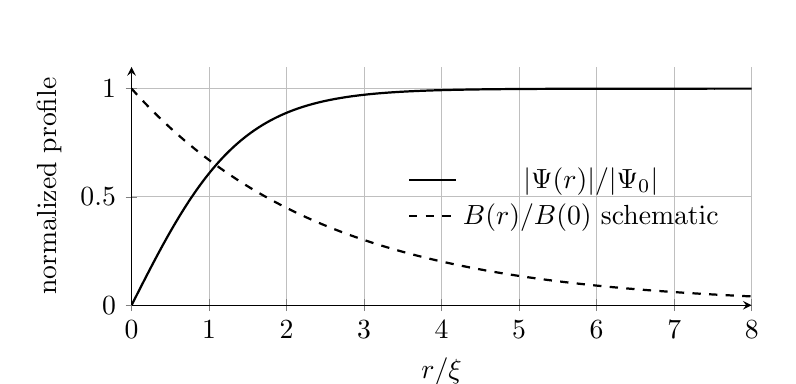
\begin{tikzpicture}
\begin{axis}[
width=0.78\textwidth,
height=0.38\textwidth,
xlabel={$r/\xi$},
ylabel={normalized profile},
xmin=0,xmax=8,
ymin=0,ymax=1.1,
axis lines=left,
grid=both,
legend style={draw=none,fill=none,at={(0.97,0.45)},anchor=east},
samples=250]
\addplot[domain=0:8,thick] {tanh(x/sqrt(2))};
\addlegendentry{$|\Psi(r)|/|\Psi_0|$}
\addplot[domain=0:8,thick,dashed] {exp(-x/2.5)};
\addlegendentry{$B(r)/B(0)$ schematic}
\end{axis}
\end{tikzpicture}
\caption{Schematic vortex profiles. The order-parameter amplitude heals over the coherence length $\xi$, while magnetic field decays over the penetration depth $\lambda$. The displayed magnetic profile is schematic, not an exact Bessel-function solution.}
\end{figure}

\begin{notebox}
\textbf{Radiation-effects relevance.} Local heating, quasiparticle bursts, and defect clusters can transiently suppress $|\Psi|$. In a type-II film under magnetic field, such suppressed regions can change vortex pinning, vortex entry, or vortex motion. Vortex motion is dissipative and can degrade superconducting resonators and qubits.
\end{notebox}

\section{Microscopic origin of GL coefficients}

GL theory was originally phenomenological, but it can be derived from BCS theory near $\Tc$. The result for a clean weak-coupling $s$-wave superconductor has the structure
\begin{align}
\alpha(T)&=\alpha_0(T-\Tc),\\
\beta&>0,\\
\frac{1}{2m^*}&\quad \text{is replaced by a gradient coefficient } K \text{ in microscopic derivations.}
\end{align}
A common microscopic GL free-energy density is written as
\begin{equation}
f=\alpha |\Delta|^2+\frac{\beta}{2}|\Delta|^4+K\left|\left(\grad-\frac{2ie}{\hbar}\Avec\right)\Delta\right|^2+\frac{B^2}{2\mu_0}.
\end{equation}
In weak-coupling BCS,
\begin{align}
\alpha&=\Nzero\frac{T-\Tc}{\Tc},\\
\beta&=\frac{7\zeta(3)\Nzero}{8\pi^2(\kB\Tc)^2},\\
K&=\frac{7\zeta(3)\Nzero(\hbar v_F)^2}{48\pi^2(\kB\Tc)^2},
\end{align}
with convention-dependent factors depending on the definition of $\Nzero$ and $\Delta$. The key point is that the same microscopic parameters that set the BCS gap also set the GL stiffness and length scales.

\subsection{How to understand the expansion}

The BCS free energy can be expanded for small $\Delta$:
\begin{equation}
F_s-F_n=a(T)|\Delta|^2+b|\Delta|^4+\cdots.
\end{equation}
At $T=\Tc$, the quadratic coefficient changes sign. The quartic term stabilizes the free energy. Spatial variation of $\Delta$ costs kinetic energy because pair correlations cannot change abruptly over distances shorter than the pair size or coherence length. That cost becomes the GL gradient term.

Thus GL theory is not arbitrary curve fitting. It is the universal long-wavelength, small-order-parameter limit of microscopic superconductivity near a continuous transition.

\section{London theory as a limiting case of GL}

If the amplitude is fixed, $|\Ord|=|\Ord_0|$, and only the phase changes, GL theory reduces to London theory. In the gauge $\theta=0$,
\begin{equation}
\Jvec_s=-\frac{(q^*)^2|\Ord_0|^2}{m^*}\Avec.
\end{equation}
Taking the curl,
\begin{equation}
\grad\times\Jvec_s=-\frac{(q^*)^2|\Ord_0|^2}{m^*}\Bvec.
\end{equation}
Using Eq.~\eqref{eq:lambda_GL},
\begin{equation}
\boxed{\grad\times\Jvec_s=-\frac{1}{\mu_0\lambdaL^2}\Bvec.}
\end{equation}
Together with Ampere's law $\grad\times\Bvec=\mu_0\Jvec_s$, this yields
\begin{equation}
\lap\Bvec=\frac{1}{\lambdaL^2}\Bvec.
\end{equation}
For a planar surface with field entering along $x$, the solution is
\begin{equation}
B(x)=B(0)e^{-x/\lambdaL}.
\end{equation}
This is the Meissner effect in its simplest continuum form.

\section{Time-dependent Ginzburg-Landau theory}

\subsection{Why static GL is not enough}

Static GL theory finds extrema of the free energy. It answers questions like:
\begin{itemize}[leftmargin=2em]
\item What is the equilibrium order-parameter profile near a boundary?
\item What is the vortex structure?
\item What is the critical field?
\end{itemize}
Radiation problems are often dynamical. A radiation event can suddenly deposit energy, create high-energy phonons, produce quasiparticles, suppress the gap, change the local temperature, or change defect/trap charge. A dynamic model must answer:
\begin{itemize}[leftmargin=2em]
\item How fast does the order parameter recover?
\item How does a normal hotspot shrink or grow?
\item How do phase gradients and currents relax?
\item How does electromagnetic gauge invariance constrain the evolution?
\end{itemize}
TDGL provides a reduced answer near regimes where a local order-parameter relaxation equation is justified.

\subsection{Gradient-flow TDGL without electromagnetic potentials}

The simplest TDGL equation is a dissipative gradient flow:
\begin{equation}
\GammaTD\pdv{\Ord}{t}=-\frac{\delta F}{\delta \Ord^*}.
\end{equation}
Using the GL variation, without electromagnetic fields,
\begin{equation}
\frac{\delta F}{\delta \Ord^*}=\alpha\Ord+\beta|\Ord|^2\Ord-\frac{\hbar^2}{2m^*}\lap\Ord.
\end{equation}
Therefore
\begin{equation}
\boxed{\GammaTD\pdv{\Ord}{t}= -\alpha\Ord-\beta|\Ord|^2\Ord+\frac{\hbar^2}{2m^*}\lap\Ord.}
\label{eq:simple_tdgl}
\end{equation}
This equation evolves $\Ord$ downhill in free energy. To verify this, compute
\begin{equation}
\dv{F}{t}=\int d^3r\left(\frac{\delta F}{\delta\Ord}\pdv{\Ord}{t}+\frac{\delta F}{\delta\Ord^*}\pdv{\Ord^*}{t}\right).
\end{equation}
If
\begin{equation}
\pdv{\Ord}{t}=-\frac{1}{\GammaTD}\frac{\delta F}{\delta\Ord^*},
\end{equation}
then
\begin{equation}
\dv{F}{t}=-\frac{2}{\GammaTD}\int d^3r\left|\frac{\delta F}{\delta\Ord^*}\right|^2\le 0
\end{equation}
for real positive $\GammaTD$. Thus the dynamics relaxes toward a GL extremum.

\subsection{Gauge-covariant TDGL}

In electromagnetic fields, ordinary $\partial_t$ is not gauge covariant. The scalar potential must appear through
\begin{equation}
D_t=\pdv{}{t}+\frac{i q^*}{\hbar}\phi.
\end{equation}
The gauge-covariant TDGL equation is
\begin{equation}
\boxed{
\GammaTD\left(\pdv{}{t}+\frac{i q^*}{\hbar}\phi\right)\Ord
=-\left[\alpha\Ord+\beta|\Ord|^2\Ord+\frac{1}{2m^*}\left(-i\hbar\grad-q^*\Avec\right)^2\Ord\right].}
\label{eq:gauge_tdgl}
\end{equation}
The current is still given by the GL current expression,
\begin{equation}
\Jvec_s=\frac{q^*\hbar}{2m^*i}\left(\Ord^*\grad\Ord-\Ord\grad\Ord^*\right)-\frac{(q^*)^2}{m^*}|\Ord|^2\Avec.
\end{equation}
The electromagnetic fields satisfy Maxwell equations or a reduced electroquasistatic or magnetoquasistatic approximation, depending on the problem.

\begin{notebox}
\textbf{Modeling warning.} TDGL is not a universal nonequilibrium BCS solver. It is most controlled near $\Tc$ and in dirty superconductors under assumptions that allow local relaxation. Millikelvin superconducting qubits often operate far below $\Tc$, so TDGL should be used carefully as a reduced phenomenological model for order-parameter suppression and recovery, not as a complete microscopic quasiparticle kinetic theory.
\end{notebox}

\section{Amplitude and phase form of TDGL}

Let
\begin{equation}
\Ord=f e^{i\theta}.
\end{equation}
For clarity, first set $\Avec=0$ and $\phi=0$. Then Eq.~\eqref{eq:simple_tdgl} gives
\begin{equation}
\GammaTD\pdv{}{t}(f e^{i\theta})=-\alpha f e^{i\theta}-\beta f^3 e^{i\theta}+\frac{\hbar^2}{2m^*}\lap(f e^{i\theta}).
\end{equation}
Use
\begin{equation}
\pdv{}{t}(f e^{i\theta})=e^{i\theta}\left(\pdv{f}{t}+if\pdv{\theta}{t}\right),
\end{equation}
and
\begin{equation}
\lap(f e^{i\theta})=e^{i\theta}\left[\lap f-f(\grad\theta)^2+i\left(2\grad f\cdot\grad\theta+f\lap\theta\right)\right].
\end{equation}
Equating real and imaginary parts gives
\begin{align}
\GammaTD\pdv{f}{t}&=-\alpha f-\beta f^3+\frac{\hbar^2}{2m^*}\left[\lap f-f(\grad\theta)^2\right],\\
\GammaTD f\pdv{\theta}{t}&=\frac{\hbar^2}{2m^*}\left[2\grad f\cdot\grad\theta+f\lap\theta\right].
\end{align}
The first equation says amplitude is suppressed by phase gradients because superflow costs kinetic energy. The second equation describes relaxation of phase texture in this purely dissipative model.

With electromagnetic fields, the phase gradients are replaced by the gauge-invariant combination
\begin{equation}
\bm{Q}=\grad\theta-\frac{q^*}{\hbar}\Avec,
\end{equation}
and the time derivative of the phase is replaced by
\begin{equation}
\Omega=\pdv{\theta}{t}+\frac{q^*}{\hbar}\phi.
\end{equation}
These combinations are invariant under gauge transformations.

\section{TDGL relaxation time near $T_c$}

Consider a spatially uniform superconductor without fields. TDGL becomes
\begin{equation}
\GammaTD\dv{\Ord}{t}=-\alpha\Ord-\beta|\Ord|^2\Ord.
\end{equation}
Above $\Tc$, $\alpha>0$, and for small $\Ord$ the cubic term is negligible:
\begin{equation}
\GammaTD\dv{\Ord}{t}=-\alpha\Ord.
\end{equation}
Thus
\begin{equation}
\Ord(t)=\Ord(0)e^{-t/\tau_{\mathrm{GL}}},
\qquad
\boxed{\tau_{\mathrm{GL}}=\frac{\GammaTD}{\alpha}.}
\end{equation}
Since $\alpha=\alpha_0(T-\Tc)$,
\begin{equation}
\tau_{\mathrm{GL}}\propto \frac{1}{T-\Tc}.
\end{equation}
The relaxation time diverges as $T\to\Tc^+$; this is critical slowing down.

Below $\Tc$, linearize around $\Ord_0$. Let $\Ord=\Ord_0+\eta$ with real amplitude perturbation and $\Ord_0^2=-\alpha/\beta$. The amplitude equation gives
\begin{equation}
\GammaTD\dv{\eta}{t}=-2|\alpha|\eta,
\end{equation}
so
\begin{equation}
\tau_{\mathrm{amp}}=\frac{\GammaTD}{2|\alpha|}.
\end{equation}
Again the time scale grows near $\Tc$.

\section{Normal current, electrochemical potential, and charge conservation in TDGL}

A practical TDGL model often includes both supercurrent and normal current:
\begin{equation}
\Jvec=\Jvec_s+\Jvec_n.
\end{equation}
A reduced normal Ohmic current is
\begin{equation}
\Jvec_n=\sigma_n\Evec=-\sigma_n(\grad\phi+\pdv{\Avec}{t}).
\end{equation}
Charge conservation requires
\begin{equation}
\pdv{\rho}{t}+\grad\cdot\Jvec=0.
\end{equation}
In many superconducting simulations, local charge neutrality or electroquasistatic constraints are imposed rather than evolving full electromagnetic waves. A common reduced condition is
\begin{equation}
\grad\cdot(\Jvec_s+\Jvec_n)=0.
\end{equation}
This closes the TDGL system for $\Ord$ and $\phi$ under a chosen gauge and boundary conditions.

\section{Nondimensional TDGL form for numerical modeling}

For finite-element or finite-difference simulation, nondimensionalization is essential. Let
\begin{equation}
\Ord=\Ord_0\psi,
\qquad
\rvec=\xiGL\rvec',
\qquad
\Avec=\frac{\hbar}{|q^*|\xiGL}\Avec',
\qquad
\phi=\frac{\hbar}{|q^*|\tau_{\mathrm{GL}}}\phi',
\qquad
 t=\tau_{\mathrm{GL}}t'.
\end{equation}
Using $\Ord_0^2=|\alpha|/\beta$ and $\xiGL^2=\hbar^2/(2m^*|\alpha|)$, the TDGL equation can be written schematically as
\begin{equation}
\left(\pdv{}{t'}+i\phi'\right)\psi=(\grad'-i\Avec')^2\psi+(1-|\psi|^2)\psi.
\label{eq:dimensionless_tdgl}
\end{equation}
The dimensionless current has the structure
\begin{equation}
\Jvec_s' = \mathrm{Im}\left[\psi^*(\grad'-i\Avec')\psi\right].
\end{equation}
The magnetic equation introduces $\kappa$:
\begin{equation}
\grad'\times\grad'\times\Avec'=\frac{1}{\kappa^2}\Jvec_s' + \text{normal-current/displacement terms depending on model}.
\end{equation}

\begin{physicsbox}
\textbf{Implementation meaning.} In a MATLAB FEM implementation, the complex field $\psi$ can be stored as two real fields, $\psi_R$ and $\psi_I$. The nonlinear term $(1-|\psi|^2)\psi$ couples them. The covariant gradient $(\nabla-i\Avec)\psi$ is the mathematical place where magnetic vector potential enters the stiffness matrix.
\end{physicsbox}

\section{Radiation perturbations in BCS, GL, and TDGL language}

\subsection{Pair breaking at the BCS level}

Radiation can create high-energy phonons, photons, and electronic excitations. If energy $2\Delta$ or greater is delivered to the superconducting condensate, pairs can be broken:
\begin{equation}
\mathrm{Cooper\ pair}+\hbar\omega\to \mathrm{QP}+\mathrm{QP},
\qquad \hbar\omega\ge 2\Delta.
\end{equation}
A reduced quasiparticle-density equation is
\begin{equation}
\pdv{n_{\mathrm{qp}}}{t}=D_{\mathrm{qp}}\nabla^2 n_{\mathrm{qp}}+G_{\mathrm{pb}}-R_{\mathrm{qp}}n_{\mathrm{qp}}^2-\frac{n_{\mathrm{qp}}}{\tau_{\mathrm{trap}}}.
\end{equation}
This equation is not TDGL. It is a quasiparticle population model. It is often more appropriate far below $\Tc$ than TDGL when the condensate amplitude remains mostly intact but nonequilibrium quasiparticles dominate device loss.

\subsection{Coefficient shifts at the GL level}

Radiation-induced disorder, heating, and defects can be represented phenomenologically by changing GL coefficients:
\begin{align}
\alpha(\rvec,t)&=\alpha_0[T(\rvec,t)-\Tc(\rvec,t)],\\
\beta(\rvec,t)&=\beta_0+\delta\beta(\rvec,t),\\
K(\rvec,t)&=K_0+\delta K(\rvec,t),\\
\sigma_n(\rvec,t)&=\sigma_{n0}+\delta\sigma_n(\rvec,t).
\end{align}
The most direct effect is local heating: if $T(\rvec,t)$ approaches or exceeds $\Tc$, then $\alpha$ changes sign and the local superconducting state is suppressed.

Defects can also reduce mean free path, modify $\Tc$, change penetration depth, create subgap states, or alter vortex pinning. A reduced model may capture these effects through spatially varying GL coefficients.

\subsection{Order-parameter recovery at the TDGL level}

If a radiation event produces a local hotspot, TDGL can model recovery by allowing $\alpha(\rvec,t)$ to return from a normal value to a superconducting value. A simple source-driven model is
\begin{equation}
\GammaTD\left(\pdv{}{t}+\frac{iq^*}{\hbar}\phi\right)\Ord
=-\alpha(\rvec,t)\Ord-\beta|\Ord|^2\Ord-\frac{1}{2m^*}\left(-i\hbar\grad-q^*\Avec\right)^2\Ord,
\end{equation}
with
\begin{equation}
\alpha(\rvec,t)=\alpha_0[T(\rvec,t)-\Tc].
\end{equation}
This couples naturally to a thermal module:
\begin{equation}
\rho_m c_p\pdv{T}{t}=\grad\cdot(k\grad T)+Q_{\mathrm{rad}}-Q_{\mathrm{e-ph}}+\cdots.
\end{equation}
In this form, radiation energy deposition drives $T$, $T$ drives $\alpha$, and $\alpha$ drives order-parameter suppression or recovery.

\section{Connection to Josephson junctions and transmons}

BCS and GL describe superconducting electrodes. A Josephson junction adds a weak link. The essential phase variable is the gauge-invariant phase difference
\begin{equation}
\delta=\theta_2-\theta_1-\frac{q^*}{\hbar}\int_1^2\Avec\cdot d\bm{\ell}.
\end{equation}
For Cooper-pair charge magnitude $2e$,
\begin{equation}
\delta=\theta_2-\theta_1+\frac{2e}{\hbar}\int_1^2\Avec\cdot d\bm{\ell}
\end{equation}
depending on sign convention. The Josephson relations are
\begin{align}
I_s&=I_c\sin\delta,\\
\hbar\dv{\delta}{t}&=2eV.
\end{align}
The Josephson energy is
\begin{equation}
E_J=\frac{\hbar I_c}{2e},
\qquad
U_J(\delta)=-E_J\cos\delta.
\end{equation}
Radiation affects Josephson devices through several channels:
\begin{itemize}[leftmargin=2em]
\item quasiparticles tunnel across the junction and cause parity switches or relaxation;
\item trapped charge changes offset charge and local electric fields;
\item local heating suppresses $\Delta$ and can reduce $I_c$;
\item defects in the tunnel barrier can act as two-level systems;
\item magnetic disturbances can change the phase bias.
\end{itemize}
At the simplest Ambegaokar-Baratoff level, the zero-temperature critical current of a tunnel junction scales with the gap:
\begin{equation}
I_c R_N=\frac{\pi\Delta}{2e},
\end{equation}
where $R_N$ is the normal-state resistance. Thus gap suppression from heating or pair breaking can directly reduce $I_c$ and therefore $E_J$.

\section{What not to confuse}

\begin{physicsbox}
\textbf{Gap versus order parameter.} In BCS theory, $\Delta$ is the pair potential and also the quasiparticle gap for an ideal isotropic $s$-wave superconductor. In GL theory, $\Psi$ is a macroscopic order parameter. Near $T_c$, $\Psi$ is proportional to $\Delta$, but they are not the same object in all regimes.
\end{physicsbox}

\begin{physicsbox}
\textbf{Quasiparticle density versus condensate density.} A quasiparticle is an excitation above the superconducting ground state. Condensate density describes the coherent paired component. Increasing quasiparticle density usually means pair breaking or excitation, not increasing superconductivity.
\end{physicsbox}

\begin{physicsbox}
\textbf{TDGL versus quasiparticle diffusion.} TDGL evolves the complex order parameter. A quasiparticle diffusion-recombination equation evolves quasiparticle number density. Both may be needed, but they are not the same equation and should not be merged without a clear approximation.
\end{physicsbox}

\section{Finite-element weak form of static GL}

Because this project uses FEM modules, it is useful to write the GL weak form. Start from the first GL equation
\begin{equation}
\alpha\Ord+\beta|\Ord|^2\Ord+\frac{1}{2m^*}\hat{\Pi}^2\Ord=0,
\qquad
\hat{\Pi}=-i\hbar\grad-q^*\Avec.
\end{equation}
A numerically convenient equivalent is obtained from the free-energy variation. Let $w$ be a complex test function. The weak form is
\begin{equation}
\int_\Omega d\Omega\left[\alpha w^*\Ord+\beta w^*|\Ord|^2\Ord+\frac{1}{2m^*}(\hat{\Pi}w)^*\cdot(\hat{\Pi}\Ord)\right]=0,
\label{eq:gl_weak}
\end{equation}
with natural boundary condition $\nvec\cdot\hat{\Pi}\Ord=0$ on insulating boundaries.

Use finite-element expansions
\begin{equation}
\Ord_h(\rvec)=\sum_{a=1}^{N}N_a(\rvec)\Ord_a,
\qquad
w_h(\rvec)=N_b(\rvec)
\end{equation}
for node $b$. The residual for node $b$ is
\begin{equation}
R_b=\int_\Omega d\Omega\left[\alpha N_b\Ord_h+\beta N_b|\Ord_h|^2\Ord_h+\frac{1}{2m^*}(\hat{\Pi}N_b)^*\cdot(\hat{\Pi}\Ord_h)\right].
\end{equation}
Since $\Ord$ is complex, one can either solve complex algebra directly or split
\begin{equation}
\Ord=\Ord_R+i\Ord_I.
\end{equation}
Then $R_b$ splits into real and imaginary residual equations. The nonlinear term is
\begin{equation}
|\Ord|^2\Ord=(\Ord_R^2+\Ord_I^2)(\Ord_R+i\Ord_I).
\end{equation}

\section{Finite-element weak form of TDGL}

For TDGL, use the gauge-covariant equation
\begin{equation}
\GammaTD D_t\Ord=-\frac{\delta F}{\delta\Ord^*}.
\end{equation}
A backward-Euler time discretization gives
\begin{equation}
D_t\Ord\approx \frac{\Ord^{m+1}-\Ord^m}{\Delta t}+\frac{i q^*}{\hbar}\phi^{m+1}\Ord^{m+1}.
\end{equation}
The weak residual at time step $m+1$ is
\begin{align}
R_b^{m+1}=&\int_\Omega d\Omega\,N_b\GammaTD\left[\frac{\Ord_h^{m+1}-\Ord_h^m}{\Delta t}+\frac{i q^*}{\hbar}\phi^{m+1}\Ord_h^{m+1}\right]\\
&+\int_\Omega d\Omega\left[\alpha N_b\Ord_h^{m+1}+\beta N_b|\Ord_h^{m+1}|^2\Ord_h^{m+1}+\frac{1}{2m^*}(\hat{\Pi}N_b)^*\cdot(\hat{\Pi}\Ord_h^{m+1})\right].
\end{align}
The first integral gives a mass matrix. The gradient term gives a gauge-covariant stiffness matrix. The cubic term gives a nonlinear reaction residual. This structure is very similar to other FEM reaction-diffusion modules in the project, except that the unknown field is complex and gauge coupled.

\section{Model-selection guidance for RadiationEffects\_proj2}

\subsection{When BCS-level modeling is the right level}

Use BCS-level quantities when the dominant question is quasiparticle generation, gap suppression, or pair-breaking thresholds. Examples:
\begin{itemize}[leftmargin=2em]
\item estimating whether a phonon spectrum can break pairs;
\item computing equilibrium quasiparticle density;
\item modeling nonequilibrium quasiparticle diffusion and recombination;
\item estimating changes in Josephson critical current from gap suppression.
\end{itemize}
A reduced model may use
\begin{equation}
\Delta(T),\qquad n_{\mathrm{qp}}(T),\qquad G_{\mathrm{pb}},\qquad R_{\mathrm{qp}},\qquad D_{\mathrm{qp}}.
\end{equation}

\subsection{When GL-level modeling is the right level}

Use GL theory when spatial order-parameter structure matters:
\begin{itemize}[leftmargin=2em]
\item superconducting film edges and holes;
\item vortex entry and pinning;
\item local suppression near defects or hotspots;
\item current crowding and depairing;
\item magnetic field penetration.
\end{itemize}
A reduced model may use
\begin{equation}
\Psi(\rvec),\qquad \xiGL,\qquad \lambdaL,\qquad \kappa,\qquad \Jvec_s.
\end{equation}

\subsection{When TDGL-level modeling is the right level}

Use TDGL when the order parameter itself is dynamically suppressed and recovers on a time scale of interest:
\begin{itemize}[leftmargin=2em]
\item hotspot recovery after radiation deposition;
\item transient phase slips in narrow wires;
\item vortex motion in a time-dependent current or thermal field;
\item qualitative condensate recovery dynamics near $\Tc$.
\end{itemize}
For millikelvin transmon modeling, TDGL should usually be treated as a phenomenological layer. Quasiparticle kinetic equations may be more appropriate for far-below-$\Tc$ nonequilibrium poisoning.

\section{Compact equation map}

\begin{center}
\renewcommand{\arraystretch}{1.25}
\begin{tabularx}{0.98\textwidth}{p{0.20\textwidth} X}
\toprule
\textbf{Theory level} & \textbf{Core equations and meaning}\\
\midrule
BCS gap & $\displaystyle 1=V\sum_{\kvec} \frac{1}{2E_{\kvec}}\tanh\left(\frac{E_{\kvec}}{2\kB T}\right)$, with $E_{\kvec}=\sqrt{\xi_{\kvec}^2+\Delta^2}$. Self-consistent microscopic pairing.\\
BCS QPs & $\displaystyle \DOS_s(E)=\DOS_n(0)|E|/\sqrt{E^2-\Delta^2}$. Gapped excitation spectrum and gap-edge singularity.\\
GL free energy & $\displaystyle F=\int d^3r\left[\alpha|\Psi|^2+\frac{\beta}{2}|\Psi|^4+\frac{1}{2m^*}|(-i\hbar\nabla-q^*\mathbf A)\Psi|^2+\frac{B^2}{2\mu_0}\right]$. Macroscopic order-parameter theory.\\
GL equation & $\displaystyle \alpha\Psi+\beta|\Psi|^2\Psi+\frac{1}{2m^*}(-i\hbar\nabla-q^*\mathbf A)^2\Psi=0$. Static equilibrium condition.\\
GL current & $\displaystyle \mathbf J_s=\frac{q^*\hbar}{2m^*i}(\Psi^*\nabla\Psi-\Psi\nabla\Psi^*)-\frac{(q^*)^2}{m^*}|\Psi|^2\mathbf A$. Supercurrent from phase stiffness.\\
TDGL & $\displaystyle \Gamma(\partial_t+iq^*\phi/\hbar)\Psi=-\delta F/\delta\Psi^*$. Gauge-covariant dissipative order-parameter dynamics.\\
\bottomrule
\end{tabularx}
\end{center}

\section{Checklist of assumptions}

\begin{enumerate}[leftmargin=2em]
\item \textbf{BCS weak coupling:} attractive interaction approximated as constant inside a phonon shell; density of states treated as constant near the Fermi surface.
\item \textbf{Isotropic $s$-wave gap:} $\Delta$ is independent of momentum. Unconventional superconductors require modified gap symmetry.
\item \textbf{Mean field:} pair fluctuations are neglected except through the self-consistent gap.
\item \textbf{GL near $T_c$:} order parameter is small, so free energy can be expanded in powers and gradients.
\item \textbf{Local GL coefficients:} material properties enter through local coefficients $\alpha$, $\beta$, $K$, and electromagnetic coupling.
\item \textbf{TDGL validity:} order-parameter dynamics is local and relaxational. Far below $T_c$, microscopic kinetic equations may be required for accurate quasiparticle nonequilibrium.
\item \textbf{Radiation coupling:} deposited energy, phonons, and defects are not automatically included in BCS/GL/TDGL; they must enter through sources, coefficient changes, boundary conditions, or coupled thermal/quasiparticle equations.
\end{enumerate}

\section{Summary}

BCS theory explains why an attractive interaction near the Fermi surface produces a superconducting ground state. The core result is a self-consistent gap $\Delta$ and a quasiparticle spectrum $E_{\kvec}=\sqrt{\xi_{\kvec}^2+\Delta^2}$. The excitation gap suppresses equilibrium quasiparticles exponentially, but radiation can create nonequilibrium quasiparticles by depositing energy above the pair-breaking threshold $2\Delta$.

GL theory translates superconductivity into a complex macroscopic order parameter $\Psi$. Its free energy contains local condensation terms, a gauge-covariant gradient energy, and magnetic-field energy. Variational minimization gives the GL equation and supercurrent. The key length scales are the coherence length $\xi$ and penetration depth $\lambda$, and their ratio $\kappa$ determines type-I versus type-II behavior.

TDGL adds time dependence by evolving $\Psi$ according to a gauge-covariant relaxation equation. It is useful for modeling order-parameter suppression and recovery, phase dynamics, and vortex motion in a reduced continuum framework. For low-temperature superconducting qubits, TDGL should usually be paired with or distinguished from quasiparticle kinetic equations, because quasiparticle poisoning can dominate even when the condensate amplitude remains nearly unchanged.

For \texttt{RadiationEffects\_proj2}, these theories provide a physically organized superconducting layer: BCS for gap and quasiparticles, GL for spatial condensate response, and TDGL for transient condensate dynamics after radiation-induced perturbations.

\section*{Recommended references for further study}
\addcontentsline{toc}{section}{Recommended references for further study}

\begin{enumerate}[leftmargin=2em]
\item M. Tinkham, \textit{Introduction to Superconductivity}. Clear physical discussion of BCS, GL, London theory, Josephson effects, and nonequilibrium superconductivity.
\item P. G. de Gennes, \textit{Superconductivity of Metals and Alloys}. Classic treatment of GL theory, boundary conditions, proximity effects, and microscopic foundations.
\item J. R. Schrieffer, \textit{Theory of Superconductivity}. Original-style microscopic presentation of BCS theory and quasiparticles.
\item A. A. Abrikosov, \textit{Fundamentals of the Theory of Metals}. Useful for superconductivity in the broader context of electron many-body theory.
\item M. Cyrot and D. Pavuna, \textit{Introduction to Superconductivity and High-$T_c$ Materials}. Useful conceptual bridge between microscopic and phenomenological treatments.
\end{enumerate}

\end{document}
